\section{Despliegue de Servicios Telemáticos}
\subsection{Escenario Desarrolado y Versiones del Software}
El escenario objetivo está compuesto por dos equipos distintos conectados a través de una red local. Para simularlo, se ha utilizado el gestor de máquinas virtuales \key{Virtual Box 6.1}.

En un equipo residen los servidores principales de los servicios. Se trata de una instancia de \key{Ubuntu 16.04 Server}. En el otro equipo se encuentra instalado \key{Ubuntu 16.04 Desktop} y cumple el papel de cliente en los servicios. Las dos máquinas virtuales disponen de una tarjeta de red virtual que simula que estuviesen conectadas a la misma red.

\subsection{Servidor DNS}
Uno de los servicios a desplegar era un servidor {\DNS} raíz. El resto de los servicios se apoyan en la resolución de nombres que aporta. Por ejemplo, para que funcione el servidor mail existen dos registros: \code{pop.sstt7628.org} y \code{smtp.sstt7628.org}.

Se eligió la implementación \key{BIND9}, que es el servidor {\DNS} más comúnmente usado en internet y el estándar de facto en sistema UNIX.

\subsubsection{Configuración}
La instalación se llevó a cabo con el gestor de paquetes de \key{Ubuntu}. La configuración depende de varios archivos de texto plano.

En el fichero \file{/etc/bind/named.conf.options} se definen las opciones globales. Se ha configurado que se acepten peticiones de hosts en la red local y que se redirijan las peticiones que no se sepan resolver al servidor {\DNS} de la Universidad de Murcia.

\begin{lstlisting}[title=Fichero \file{/etc/bind/named.conf.options}]
// Para leer todo acerca a la configuración:
// https://www.zytrax.com/books/dns/ch7/
options {
    directory "/var/cache/bind";

    allow-query {        // Hosts que tienen permitido realizar consultas
    	192.168.56.0/24; // Red local de la práctica
    };

    forwarders {    // Direcciones IP de servidores dns para consultas desconocidas.
    	155.54.1.1; // Dirección IP de los servidores DNS de la universidad.
    	155.54.1.2; // Obtenida con el comando dig -t ns um.es
    };

    recursion yes;  // Habilita la recursión para resolver consultas anidadas.
                    // Por ejemplo: www.sstt7628.org (org, sstt7628.org, www.sstt7628.org)

    dnssec-validation auto;

    auth-nxdomain no;     # conform to RFC1035
    listen-on-v6 { any; };
};
\end{lstlisting}

El fichero \file{/etc/bind/named.conf.local} sirve para configurar las zonas que conoce el servidor. Basta con poner que se trata de una zona manejada por nuestro servidor (\key{type master}) y definir un fichero de zona que debemos localizar en la carpeta \file{/etc/bind}. Es habitual, si hay pocos ficheros de zona, que el nombre de los ficheros de zona debe comenzar por \key{db} y no se incluyan dentro de ninguna subcarpeta, pero no es obligatorio.

\begin{lstlisting}[title=Fichero \file{/etc/bind/named.conf.local}]
zone "sstt7628.org." IN {
    type master; // El servidor lee la información de un fichero de zona local
                 // y responde de forma autoritativa.
    file "/etc/bind/db.sstt7628.org.zone"; // El fichero de zona
}
\end{lstlisting}

En el fichero de zona (\key{/etc/bind/db.sstt7628.org.zone}) se configuraron los valores asociados a nuestro dominio, como el \key{TTL} (\textit{time to live}). En mi caso he definido varios registros, entre ellos dos registros de correo electrónico, que se utilizan en el resto de apartados.
\begin{lstlisting}[title=Fichero \file{/etc/bind/db.sstt7628.org.zone}]
; Toda la información de configuración de los ficheros de zona en
; https://www.zytrax.com/books/dns/ch8/
$ORIGIN    sstt7628.org. ; Especificamos que a los nombres que acaben sin un punto
                         ; se les añada esta ruta
$TTL    3600
@         IN    SOA     sstt7628.org. root.sstt7628.org. (
                             1        ; Serial
                          3600        ; Refresh
                          1800        ; Retry
                        604800        ; Expire
                          3600)       ; Negative Cache TTL
;
@         IN    NS      localhost.
cliente   IN    A       192.168.56.101
servidor  IN    A       192.168.56.104
www       IN    CNAME   servidor
web       IN    CNAME   servidor
mail      IN    A       192.168.56.104
@         IN    MX 10   mail
smtp      IN    CNAME   mail
pop       IN    CNAME   mail
\end{lstlisting}

Por otro lado, además de registrar el servidor {\DNS} hay que configurar los hosts para que hagan peticiones a este servidor.

La configuración de dominios {\DNS} se encuentra en el fichero \file{/etc/resolv.conf}. No obstante, los cambios que hagamos sobre este fichero se perderán al reiniciar el ordenador, porque es un fichero generado automáticamente. En su lugar, podemos editar el fichero \file{/etc/resolvconf/resolv.conf.d/head}, que se copia al principio durante la generación. Para añadir un servidor {\DNS} basta con añadir la línea

\begin{center}\code{nameserver 192.168.56.104}.\end{center}

Podemos evitar reiniciar el sistema para ver los cambios ejecutando la orden \code{resolvconf -u}.

\subsubsection{Capturas Wireshark}
A continuación (\cref{img-cap-dns}) se muestra un trozo de la captura Wireshark adjunta donde se ve una consulta {\DNS}.

\begin{figure}[h]
    \centering
    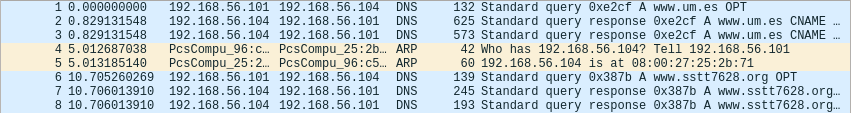
\includegraphics[width=0.95\textwidth]{tests/capture-dns.png}
    \caption{Dos consultas {\DNS}}
    \label{img-cap-dns}
\end{figure}

\subsection{Correo {\SMTP/\POP}}
Se ha desplegado también un servicio de correo electrónico {\SMTP/\POP} mediante las implementaciones \key{exim} y \key{dovecot}. El procedimiento ha sido el explicado en las sesiones de prácticas.

\subsubsection{Usuarios de correo}
Se crearon dos usuarios de correo con nombres \code{nombre1_49277628@sstt7628.org} y \code{nombre2_49277628@sstt7628.org} como pedía la práctica. Con la configuración vista en clase, basta con registrar ambos usuarios en el sistema y el directorio de correo (\key{Mailbox}) se crea automáticamente.

Para verificar el funcionamiento se se utilizó el gestor de correo \key{Thunderbird} (en el cliente) y se enviaron varios correos de una a otra.

\subsubsection{Capturas Wireshark}
A continuación (\cref{img-cap-mail}) se muestra un trozo de la captura Wireshark adjunta donde se muestran los mensajes intercambiados para el envío de un correo electrónico.

\begin{figure}[h]
    \centering
    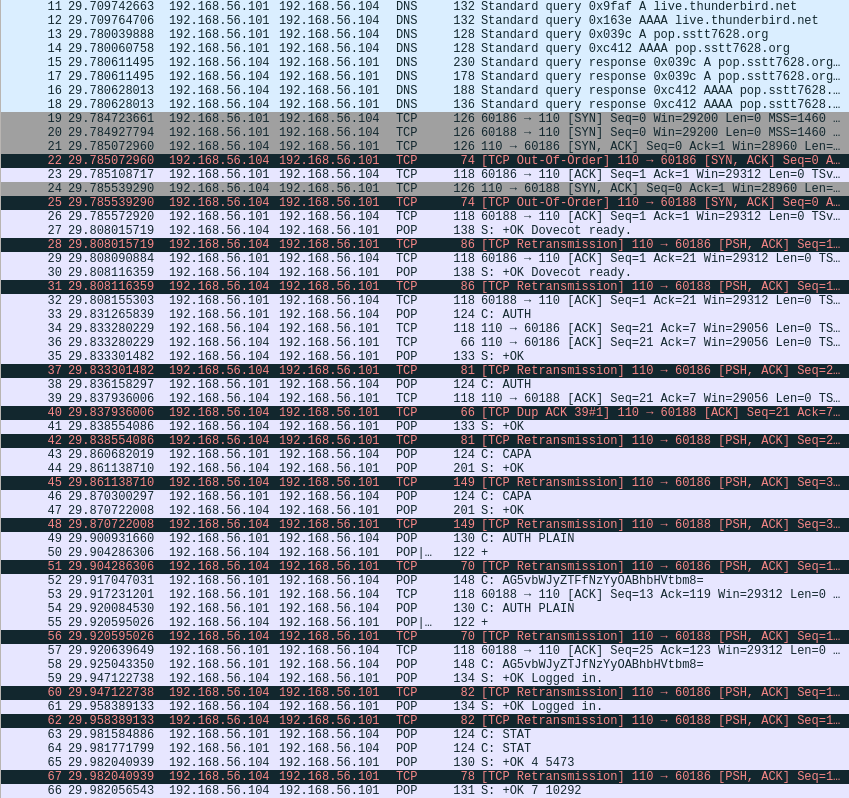
\includegraphics[width=0.95\textwidth]{tests/capture-mail.png}
    \caption{Tráfico generado por Thunderbird}
    \label{img-cap-mail}
\end{figure}

\subsection{Servidor {\HTTP} y {\HTTPs} basado en \key{Apache}}
El grueso del trabajo era implementar el servidor {\HTTP} descrito en la primera sección. No obstante, también hemos tenido que configurar un servidor \key{Apache} que recibiese peticiones {\HTTP} (en el puerto $80$) y {\HTTPs} (en el puerto $443$).

\subsubsection{Configuración}
La configuración se lleva a cabo, una vez más, a través de ficheros de configuración del sistema. Para usar \key{Apache} hay que configurar \key{Virtual Hosts} a través de los siguientes pasos.

\begin{enumerate}
\item Se crea el fichero del sitio \file{/etc/apache2/sites-available/sitio.conf} (Apache incluye ficheros de ejemplo que se pueden utilizar como base). Para la práctica se ha configurado ambos \key{Virtual Hosts} en el mismo fichero porque corresponden al mismo sitio.
\item Se activa el fichero con el comando \code{a2ensite}, que entre otras cosas crea un enlace dinámico a nuestro fichero en la carpeta \file{/etc/apache2/sites-available/}.
\item Y se recarga el servicio de apache (\code{service apache2 reload}), tras lo cual ya podemos acceder.
\end{enumerate}

Si no disponemos de un servicio de {\DNS} que resuelva los nombres de nuestros sitios, podemos añadir una entrada al fichero \file{/etc/hosts}, que sirve para registrar traducciones estáticas en \key{Linux}. En mi caso, instalé \key{Apache} antes de configurar \key{BIND} y ese fue el procedimiento inicial.

El servidor {\HTTP} se protegió mediante usuario y contraseña siguiendo los siguientes pasos.

\begin{itemize}
\item Configuramos el virtual host {\HTTP} de \key{Apache} para restringir la entrada a un grupo de usuarios registrados en ficheros de configuración de \key{Apache}. Es decir, para utilizar un login y contraseña.

\begin{lstlisting}[title=Primera parte del fichero \file{/etc/apache2/sites-available/sstt7628.conf}]
<VirtualHost *:80>
	ServerName www.sstt7628.org

	ServerAdmin admin@sstt7628.org
	DocumentRoot /var/www/sstt7628

	<Directory /var/www/sstt7628>
		AllowOverride AuthConfig
		AuthType Basic
		AuthName "Restricted access to group sstt7628"
		AuthBasicProvider file
		AuthUserFile /etc/apache2/passwords
		AuthGroupFile /etc/apache2/groups
		Require Group sstt7628
			Order allow,deny
			allow from all
	</Directory>

	ErrorLog ${APACHE_LOG_DIR}/error.log
	CustomLog ${APACHE_LOG_DIR}/access.log combined
</VirtualHost>
\end{lstlisting}

\item Los usuarios se crean con el comando \code{htpasswd -c /etc/apache2/passwords sstt7628} y se registran en el grupo añadiendo un fichero \file{groups} en la carpeta donde se encuentre el fichero de usuarios con el siguiente formato
\begin{lstlisting}[title=Fichero \file{/etc/apache2/groups}]
    sstt7628: sstt7628
\end{lstlisting}

\item La configuración de usuarios requiere del módulo \code{authz_groupfile} de \key{Apache}. No hace falta instalarlo en \key{Ubuntu}. Basta con ejecutar el comando \code{a2enmod authz_groupfile} para habilitarlo.
\end{itemize}


\subsection{Certificación {\HTTPs} a través de \key{OpenSSL}}
La configuración del servidor {\HTTPs} es más complicada y requiere que una entidad certificadora firme (en el sentido utilizado en informática para claves públicas y privadas) los certificados que utiliza el protocolo.

Aunque no se ha desplegado una entidad certificadora en el servidor (lo que tendría sentido sería que estuviese en un tercer ordenador), se ha simulado el proceso ejecutando los comandos de la herramienta \key{OpenSSL} tal cual vimos en las clases de prácticas y se encuentra documentado en las diapostivas.

% He utilizado el directorio `~/CAentity`.
% Para generar el primer certificado de la CA he utilizado password como palabra de paso y ca.sstt7628.org como common name.

Una vez generadas las claves para ambos dispositivos y configurado el navegador web del cliente, \key{Firefox} para que reconociese a la entidad certificadora, se configuró el servidor {\HTTPs} en el fichero \file{/etc/apache2/sites-available/sstt7628.conf}.

\begin{lstlisting}[title=Segunda parte del fichero \file{/etc/apache2/sites-available/sstt7628.conf}]
<VirtualHost *:443>
	ServerName www.sstt7628.org

	ServerAdmin admin@sstt7628.org
	DocumentRoot /var/www/sstt7628

	# Authentication Configuration
	SSLEngine on
	# Los ficheros de claves han sido generados usando OpenSSL.
	SSLCertificateFile		/home/alumno/CAentity/servercert.pem
	SSLCertificateKeyFile	/home/alumno/CAentity/serverkey.pem
	SSLCACertificateFile	/home/alumno/CAentity/cacert.pem

	SSLVerifyClient			require
	SSLVerifyDepth			10
</VirtualHost>
\end{lstlisting}

\subsubsection{Capturas Wireshark}
A continuación (\cref{img-cap-http,img-cap-https}) se muestra un trozo de la captura Wireshark adjunta donde se muestra primero un acceso al servidor web vía {\HTTP} y después vía {\HTTPs}.

\begin{figure}[h]
    \centering
    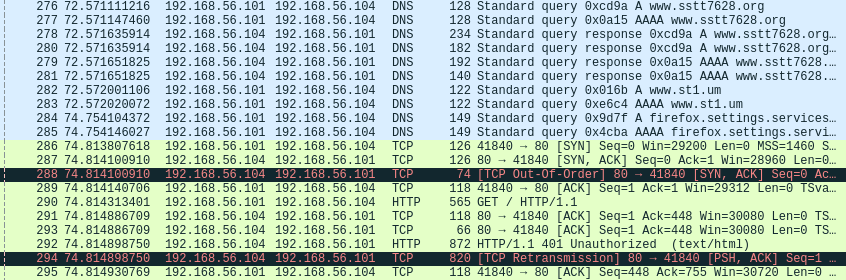
\includegraphics[width=0.95\textwidth]{tests/capture-http.png}
    \caption{Tráfico generado por \key{Firefox} con la petición {\HTTP}}
    \label{img-cap-http}
\end{figure}

\begin{figure}[h]
    \centering
    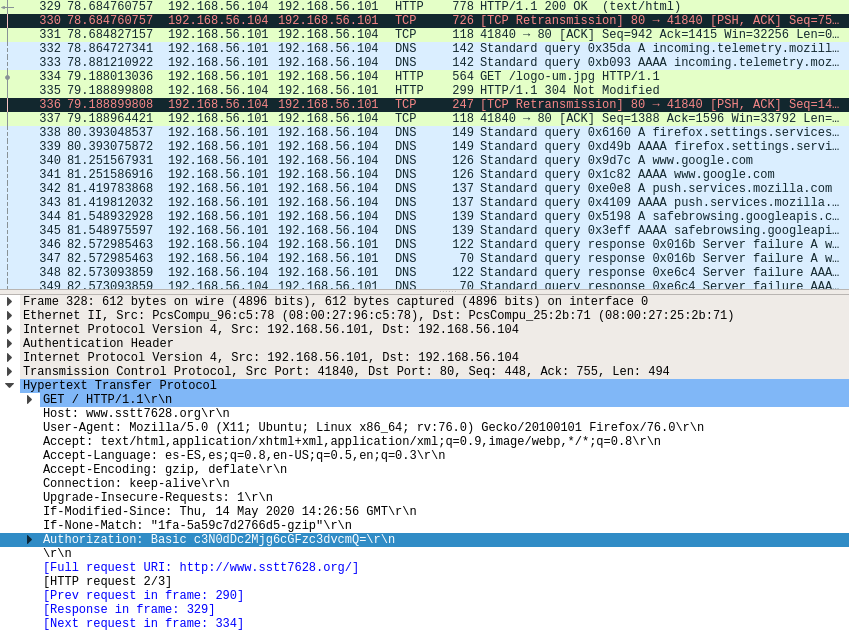
\includegraphics[width=0.95\textwidth]{tests/capture-https.png}
    \caption{Tráfico generado por \key{Firefox} con la petición {\HTTPs}}
    \label{img-cap-https}
\end{figure}


\subsection{IPsec con \key{Strongswan}}
Por último, se pedía implementar el protocolo {\IPsec} para proteger los paquetes {\IP} entre ambos dispositivos. Los requisitos eran utilizar \key{IKEv2} para el establecimiento del canal y operar en modo túnel con autentificación a través de la cabecera \key{AH}, pero sin encriptación. Para ello, se podían utilizar los certificados de identidad que utilizamos para la conexión {\HTTPs}.

Se ha hecho uso de \key{Strongswan}, una implementación \textit{Open Source} de {\IPsec}. Como en el resto de casos, la instalación se ha llevado a cabo a través del gestor de paquetes de \key{Ubuntu}, \code{apt}.

\subsubsection{Configuración}
La configuración de los canales se puede escribir en el fichero \file{/etc/ipsec.conf} de cada host.

\begin{lstlisting}[title=Fichero \file{/etc/ipsec.conf} del servidor]
config setup

conn %deault # Valores por defecto para las conexiones
	ikelifetime=60m
	keylife=20m
	rekeymargin=3m
	keyingtries=1
	mobike=no
	keyexchange=ikev2
	authby=pubkey

conn host-host # Conexión host-host de la práctica
	left=192.168.56.104 # IP del servidor
	leftcert=/etc/ipsec.d/certs/servercert.pem # Clave pública generada con OpenSSL
	leftid="C=ES, ST=Murcia, O=UMU, OU=sstt7628, CN=www.sstt7628.org"
	right=192.168.56.101 # IP del cliente
	rightid="C=ES, ST=Murcia, O=UMU, OU=sstt7628, CN=emilio49277628"
	type=tunnel
	ah=sha256
	auto=start
\end{lstlisting}

\begin{lstlisting}[title=Fichero \file{/etc/ipsec.conf} del cliente]
config setup

conn %deault # Valores por defecto para las conexiones
	ikelifetime=60m
	keylife=20m
	rekeymargin=3m
	keyingtries=1
	mobike=no
	keyexchange=ikev2
	authby=pubkey

conn host-host # Conexión host-host de la práctica
	left=192.168.56.101 # IP del cliente
	leftcert=/etc/ipsec.d/certs/servercert.pem # Clave pública generada con OpenSSL
	leftid="C=ES, ST=Murcia, O=UMU, OU=sstt7628, CN=emilio49277628"
	right=192.168.56.104 # IP del servidor
	rightid="C=ES, ST=Murcia, O=UMU, OU=sstt7628, CN=www.sstt7628.org"
	type=tunnel
	ah=sha256
	auto=start
\end{lstlisting}

En la configuración se puede ver que se ha seleccionado el modo túnel y que se utiliza el protocolo sin encriptación. Concretamente, la línea \code{ah=sha256} especifica que no se utilice encriptación \key{ESP}, el modo predeterminado en \key{Strongswan}. \key{sha256} es una función de hash que se utiliza para asegurar la integridad de los paquetes en la cabecera \key{AH}. Hay muchas opciones disponibles, y he elegido esta función por ser bastante común.

Por último, hay que modificar otro fichero, \file{/etc/ipsec.secrets}, que contiene la información delicada. Lo que hay que incluir en él es la ruta al fichero que contiene la clave privada.

\begin{lstlisting}[title=Fichero \file{/etc/ipsec.secrets} del cliente]
: RSA /etc/ipsec.d/private/clientkey.pem
\end{lstlisting}

\subsubsection{Capturas Wireshark}
A continuación (\cref{img-cap-ping}) se muestra un trozo de la captura Wireshark adjuntada donde se ve que los mensajes originados por un ping de una máquina a otra incluyen la cabecera \key{AH} de {\IPsec}.

\begin{figure}[h]
    \centering
    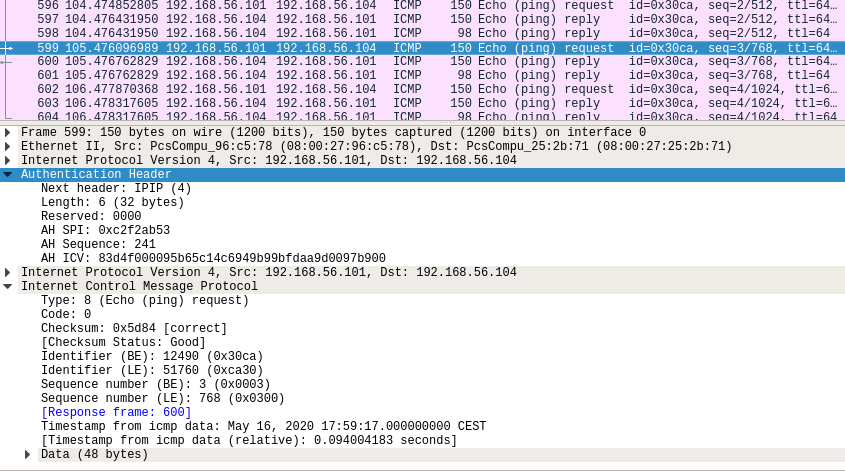
\includegraphics[width=0.95\textwidth]{tests/capture-ping.png}
    \caption{Tráfico generado por el comando \code{ping}. Se ve la cabecera \key{AH}.}
    \label{img-cap-ping}
\end{figure}

